\graphicspath{{img/intro/out}{img/intro}}

\chapter{Introduction}
\label{ch:intro}

\section{Artificial Intelligence}
\label{sec:artificial-intelligence}
Artificial Intelligence (AI) is a broad subject of study that can be defined in different ways~\cite[chapter 1]{russell_artificial_2021}.
John McCarthy, often called the “father of AI”~\cite{wiki_ai_2023, woo_fatherofai_2014, andresen_fatherofai_2002}, defines it as “the science and engineering of making intelligent machines”~\cite{stanford-whatisai}, where intelligence means “the computational part of the ability to achieve goals in the world”~\cite{stanford-whatisai}.
AI is sometimes mistakenly used interchangeably with Machine Learning.
Machine learning is a subset of AI concerned with enabling AI systems to learn from experience~\cite[chapter 1]{russell_artificial_2021}.
Machine learning enables the development of large-scale AI systems as they are used today.
\\
The study of artificial intelligence was first proposed by McCarthy et al. in late 1955 \cite{mccarthy_proposal_1955}.
It went through two major hype cycles in the sixties and the eighties~\cite{googlengram_ai, wiki_ai_2023, sitnflash_history_2017} followed by phases of “AI winter”.
The current (as of early 2024) AI boom, sometimes also called “AI spring”~\cite{aispring} was started by groundbreaking advances in speech recognition~\cite{hinton_deep_2012} and image classification~\cite{krizhevsky_imagenet_2012} in 2012~\cite{google_decade_2021, house_2012_2019} and reached the public at the latest in late 2022, following the release of ChatGPT~\cite{openai_chatgpt_intro}, a multipurpose AI-chatbot, open to everyone~\cite{openai_chatgpt}.
\\
These breakthroughs are made possible mainly by advancements in the field of machine learning, enabling AI systems to learn from huge amounts of data.
In addition, the exponential increase in computation and storage capabilities as predicted by Moore's Law~\cite{mooreslaw} and algorithms like backpropagation~\cite{rumelhart_learning_1986} allowed incorporating large amounts of data into machine learning models in realistic amounts of time.
\\
Today, AI systems are indispensable in many areas such as web search engines~\cite{google_howweuseai}, recommendation systems~\cite{burke_recommender_2011}, human speech recognition and generation~\cite{elevenlabs, hinton_deep_2012}, image recognition and generation~\cite{midjourney, krizhevsky_imagenet_2012} and personal assistants~\cite{openai_chatgpt_intro} and surpasses humans in high-level strategy games like go and chess~\cite{silver_mastering_2016, silver_mastering_2017} as well as other video games~\cite{piper_ai_2019}.

\section{Intelligent Matter, Machine Learning and Physics}
\label{sec:intelligent-matter}
Classical statistical physics is mostly concerned with systems in thermodynamic equilibrium. It studies ensembles of equilibrium systems to derive macroscopic properties from microscopic interactions. Non-equilibrium statistical mechanics studies systems that are not in thermodynamic equilibrium but are instead driven by imbalances \cite{wiki_statistical_2024}. Simple examples include the physical description of chemical reactions or systems with a steady flow of heat or particles between two baths. In nature, however, most systems are far from equilibrium \cite{fodor_how_2016}. These systems cannot be described by classical statistical mechanics and require new theoretical frameworks \cite{fodor_how_2016}. Almost all living systems fall under this category: From microscopic objects such as molecular motors, living cells and bacterial colonies to macroscopic objects such as flocks of birds or schools of fish \cite{cichos_machine_2020,fodor_how_2016}, all living systems consist of many interacting parts that draw energy from their local environment to perform mechanical work \cite{popkin_physics_2016}. These components can be simple on their own, but when they interact with each other, they can form complex structures and patterns and often exhibit highly intelligent behavior \cite{popkin_physics_2016,kaspar_rise_2021}.


The study of these systems is called \textit{active matter} research \cite{kaspar_rise_2021}. Active matter describes any kind of matter that exhibits dynamic behavior and can adapt to external stimuli \cite{kaspar_rise_2021}. It can be further distinguished from \textit{intelligent matter}, a subset of active matter that learns from and interacts with its environment \cite{kaspar_rise_2021}. Active matter research is a relatively new field of study, with the popularity of the subject beginning to rise in the mid-1990s \cite{popkin_physics_2016}. 


Modeling and replicating such systems would be of great scientific interest, as it could lead to a quantitative, mathematical theory of still-mysterious biological processes \cite{popkin_physics_2016}, but it also has great potential for real-world applications in fields such as robotics, material science and computational research. Groups of intelligent robots such as the \enquote{Kilobots} introduced by Rubenstein et al. \cite{rubenstein_kilobot_2012} can work together to complete tasks that would be impossible for a single robot, similar to how a colony of ants builds nests and transports food \cite{rubenstein_kilobot_2012}. Intelligent matter could also be used to create adaptive artificial skins \cite{kaspar_rise_2021} or smart clothing that changes its insulation properties or transparency based on the environment \cite{fernandez-carames_towards_2018}.\\
Another interesting aspect of active matter systems that was also one of the initial motivations for research in this field is the computational efficiency of these systems \cite{kaspar_rise_2021}. The human brain manages to perform complex cognitive tasks while consuming only a small amount of energy compared to modern computers \cite{balasubramanian_brain_2021}. Intelligent matter research aims to replicate nature's way of information processing to find new, more efficient ways of computing \cite{kaspar_rise_2021}. 


Machine learning can be used in different ways to study active matter systems. For one, it can be used to analyze data from active matter experiments. Applications include tracking objects in active matter data \cite{cichos_machine_2020}, analyzing time series data \cite{cichos_machine_2020} or finding connections between genetic code and emergent bacterial behavior \cite{cichos_machine_2020}.\\
Another interesting application of machine learning in active matter research is the use of machine learning to simulate new forms of active matter. Oftentimes, the rules that govern the behavior of the individual components of an active matter system are very simple, but the interactions between these components can lead to complex behavior that is hard to predict. Machine learning can be used to explore a new form of active matter where the large number of components is combined with intelligent behavior already at the microscopic level. While systems with a large number of simple components, such as the Kilobots or DNA molecules, have been studied previously, and the same is true for systems with a small number of very intelligent components, such as self-driving cars or Boston Dynamics' \enquote{Spot} \cite{bostondynamics_spot_2024,koval_experimental_2022}, this combination of a large number of intelligent components is a fairly new field of study in active matter research and especially in physics. 


While many aspects of collective human behavior are studied by the field of sociology, and studies exist on the collective behavior of animals such as the flocking of birds, the schooling of fish and krill and the herding of mammals \cite{wiki_collective_2024}, the topic is still relatively unexplored in physics. A straightforward way of studying collective behavior in active matter systems is to use agent-based modeling (ABM). In ABM, the individual units of a system (agents) are modeled and simulated to capture the emergent phenomena arising from their interaction when the simulation is run \cite{bonabeau_agent-based_2002}. This is often easy to implement while enabling a rich description of the system \cite{bonabeau_agent-based_2002}. For many systems, ABM is the most natural way of modeling them, as it recreates complex behavior from the bottom up. When modeling traffic jams or supermarket shoppers for example, it is straightforward to model the individual cars or shoppers and their interactions, but it would be very difficult to model the top-level dynamics of the system directly \cite{bonabeau_agent-based_2002}.


Popular examples of systems where highly complex behavior emerges from simple rules are cellular automata like Conway's Game of Life \cite{bays_introduction_2010,gotts_emergent_2010}, which has even been shown to be Turing-complete \cite{rendell_turing_2002}. These systems typically consist of a grid of cells that can be in a finite number of states (e.g. occupied or unoccupied) and a set of rules that determine the state of each cell in the next time step based on the state of the cell and its neighbors in the current time step. Conway's Game of Life for example has only four basic rules, but new patterns and structures are still being discovered today, more than 50 years after its invention \cite{noauthor_elementary_nodate}.\\
This thesis will use a similar grid-based system, but instead of defining the rules of the system manually, agents in the system will learn an optimal set of rules using deep reinforcement learning with neural networks, also allowing different agents to learn different rules. This is a fairly new approach in the study of active matter systems.


\section{Stochastic Processes and Markov Chains}
\label{sec:stochastic-processes}
\begin{figure}[h]
    \centering
    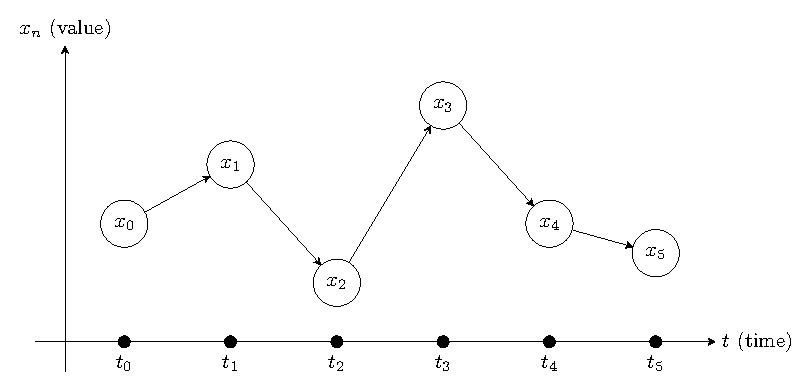
\includegraphics[width=\textwidth]{stoch_proc.pdf}
    \caption{A stochastic process is an ordered collection of random variables $x_t$ indexed by time $t$.}
    \label{fig:stochastic-processes}
\end{figure}
This section will briefly lay out the mathematical framework of stochastic processes and Markov chains. Section \ref{subsubsec:mdp} will later build on this framework to explain the mathematical foundations of reinforcement learning using Markov decision processes. The derivations in this chapter closely follow \cite[chapter 2.2]{tauber_critical_2014}.


A \textit{stochastic process} is an ordered sequence of values $x_n=x(t_n)$ of a random variable $x\in\mathcal{S}$ indexed by (possibly discrete) time $t_n\in\mathcal{T}$ (Fig. \ref{fig:stochastic-processes}). The probability of observing such a sequence of $n$ values is given by the \textit{$n$-point probability distribution}
\begin{align}
    P_n: \mathcal{S}^n \times \mathcal{T}^n &\rightarrow [0,1] \\
    (x_1, t_1; x_2, t_2; \dots; x_n, t_n) &\mapsto P_n(x_1, t_1; x_2, t_2; \dots; x_n, t_n) \text{,}
    \label{eq:n-point-probability-distribution}
\end{align}
which is normalized:
\begin{equation}
    \int dx_1 \dots \int dx_n P_n(x_1, t_1; x_2, t_2; \dots; x_n, t_n) = 1 \text{,}
    \label{eq:n-point-probability-distribution-normalized}
\end{equation}
and obeys the \textit{hierarchy rule}
\begin{equation}
    \int dx_n P_n(x_1, t_1; x_2, t_2; \dots; x_n, t_n) = P_{n-1}(x_1, t_1; x_2, t_2; \dots; x_{n-1}, t_{n-1}) \text{.}
    \label{eq:hierarchy-rule}
\end{equation}
Time averages, moments and correlations are defined in the usual way:
\begin{align}
    \langle x(t)^n \rangle &= \int dx x^n P_1(x, t) \text{,} \label{eq:moments} \\
    \langle x(t_1) \dots x(t_n) \rangle &= \int dx_1 \dots \int dx_n x_1 \dots x_n P_n(x_1, t_1; \dots; x_n, t_n) \text{.} \label{eq:correlations}
\end{align}
The same goes for conditional probabilities:
\begin{equation}
    P_{m|k}(x_{k+1}, t_{k+1}; \dots; x_{k+m}, t_{k+m} | x_1, t_1; \dots; x_k, t_k) = \frac{P_{m+k}(x_1, t_1; \dots; x_{k+m}, t_{k+m})}{P_k(x_1, t_1; \dots; x_k, t_k)} \text{.}
    \label{eq:conditional-probability}
\end{equation}
A stochastic process is called \textit{stationary} if its $n$-point probability distribution is invariant under time translations:
\begin{equation}
    P_n(x_1, t_1; \dots; x_n, t_n) = P_n(x_1, t_1 + \tau; \dots; x_n, t_n + \tau) \text{.}
    \label{eq:stationary-process}
\end{equation}
A sequence $x_{k+1}, x_{k+2}, \dots, x_{k+n}$ can be \textit{statistically independent} of the preceding sequence $x_1, x_2, \dots, x_k$:
\begin{equation}
    P_{n|k}(x_{k+1}, t_{k+1}; \dots; x_{k+n}, t_{k+n} | x_1, t_1; \dots; x_k, t_k) = P_n(x_{k+1}, t_{k+1}; \dots; x_{k+n}, t_{k+n}) \text{.}
    \label{eq:independence}
\end{equation}
In that case, the $n$-point probability distribution factorizes:
\begin{equation}
    P_n(x_1, t_1; \dots; x_{k+n}, t_{k+n}) = P_k(x_1, t_1; \dots; x_k, t_k) P_n(x_{k+1}, t_{k+1}; \dots; x_{k+n}, t_{k+n}) \text{.}
    \label{eq:factorization}
\end{equation}
In the special case where the value of the random variable $x$ at time $t_{k+1}$ only depends on the value of $x$ at time $t_k$, the process is called \textit{Markovian} and the process is called a \textit{Markov process} or \textit{Markov chain}. In that case, the conditional probability distribution simplifies to:
\begin{equation}
    P_{1|n-1}(x_n, t_n | x_1, t_1; \dots; x_{n-1}, t_{n-1}) = P_{1|1}(x_n, t_n | x_{n-1}, t_{n-1}) \text{.}
    \label{eq:markov-chain}
\end{equation} 
Markov Chains are fully characterized by their initial probability distribution $P_1(x_1, t_1)$ and their \textit{transition probabilities} $P_{1|1}(x_{j+1}, t_{j+1} | x_j, t_j)$. Using the definition of conditional probability (eq. \ref{eq:conditional-probability}) and the Markov property (eq. \ref{eq:markov-chain}), one can derive the \textit{Chapman-Kolmogorov equation} \cite[page 59]{tauber_critical_2014}:
\begin{equation}
    P_{1|1}(x', t' | x, t) = \int d\bar{x} P_{1|1}(x', t' | \bar{x}, t') P_{1|1}(\bar{x}, t' | x, t) \text{,}
    \label{eq:chapman-kolmogorov}
\end{equation}
which states that the transition from $x$ to $x'$ can be split into an arbitrary number of intermediate steps that only depend on the last step.
\\
For continuous-time Markov chains, one can derive the \textit{master equation} \cite[page 60]{tauber_critical_2014}:
\begin{equation}
    \frac{\partial}{\partial t} P_1(x, t) = \int d\bar{x} \left[ P_1(\bar{x}, t) W(\bar{x} \rightarrow x, t) - P_1(x, t) W(x \rightarrow \bar{x}, t) \right] \text{,}
    \label{eq:master-equation}
\end{equation}
where we introduced the \textit{transition rate} $W(x \rightarrow \bar{x}, t)$ from $x$ to $\bar{x}$ at time $t$. When we interpret the values of $x$ as the states of a system (as we will do in section \ref{subsubsec:mdp}, calling them \textit{states} $s$), the master equation can be interpreted as the balance of \textit{gain} and \textit{loss} of the probability to be in state $x$. Probability is gained when the system transitions from any other state $\bar{x}$ to $x$ and lost when the system transitions from $x$ to any other state $\bar{x}$.


One could continue building this powerful framework of stochastic processes and Markov chains by showing that all important properties of the probability distribution are preserved under time evolution and by introducing relevant quantitative measures such as the time-dependent \textit{entropy} and their respective evolutions as is done in \cite[chapter 2.2]{tauber_critical_2014}. However, this is beyond the scope of this thesis as the reinforcement learning problem treated in this thesis instead builds on the framework of discrete-time Markov decision processes, which will be introduced later in section \ref{subsubsec:mdp}.

\chapter{Neural Networks}
\label{ch:neural-networks}
\section{Overview}
\label{sec:overview}
At the heart of almost all the technologies mentioned in section \ref{sec:artificial-intelligence} are deep artificial neural networks.
The next section will outline the mathematical details of how these systems work and learn.
Although the comparison of artificial neural networks, from now on just called “neural networks”, to their biological counterpart can be criticized as oversimplifying the inner workings of biological brains~\cite[chapter 1.1]{aggarwal_neural_2018}, the architecture of neural networks is heavily inspired by how decision-making and learning work in the human brain~\cite[chapter 1.1]{aggarwal_neural_2018, mit_nnexplained}.
I will illustrate the basic principles of neural networks with the example of a network that detects the gender of a person by looking at pictures.


A neural network consists of several layers of artificial neurons, called \textit{nodes}.
In a \textit{fully connected} network, each node is connected to every node in the next layer.
The connection strengths are called \textit{weights}.
An image of a person can be fed into the network by setting the \textit{activation} values of the first layer of the network, the \textit{input layer}, to the individual pixel values of the image.
This information is then fed forward through the layers of the network until the \textit{output layer} is reached.
If a network has at least one layer in between the input and output layer, it is called a \textit{deep neural network}.
These intermediate layers are called \textit{hidden layers}.
If the outputs of each layer are only connected to the inputs of the next layer, the network is called a \textit{feedforward neural network}.
If \textit{feedback} connections are allowed, the network is called a \textit{recurrent neural network}.
\\
In our example, the output layer should consist of only two nodes.
If the activation of the first node is larger than the activation of the second node, the network thinks that the person in the picture is a male.
If on the other hand, the second node has a larger activation, the network classifies this person as female~\cite[chapter 1.2]{aggarwal_neural_2018}.


In order to make accurate predictions, a reasonable set of network parameters (weights) has to be found.
This is done by training the network with pre-classified images.
After an image has been processed by the network, the output is compared to the correct classification, and the network parameters are updated in a way that would improve the network output if the same image was to be processed again~\cite[chapter 1.2]{aggarwal_neural_2018,ibm_nn}.
\\
This is similar to how humans learn from experience.
If we were to misclassify a person's gender, the unpleasant social experience that may come with that mistake would cause us to update our internal model of what different genders look like to not make the same mistake again.


One of the main strengths of neural networks is their ability to \textit{generalize}~\cite{gonfalonieri_understand_2020}.
When a network is trained on a large enough set of examples, it gains the ability to generalize this knowledge to examples that were previously unseen.
The gender classification network from our example doesn't just memorize the genders of the people it has seen, but instead learns about the features that help to identify the gender of a random person.


The problem of image classification is a rather complex one. One wouldn't typically think of it as finding a function that maps the values of each input pixel to the classification output.
But even very complex problems can be modeled by equally complex functions.
The universal approximation theorem states, that a feedforward neural network with at least one hidden layer with appropriate activation functions (see~\ref{subsec:activation-functions} for details) can approximate any continuous function if given enough nodes~\cite[chapter 6.4.1]{goodfellow_deep_2016}.
That's why training a neural network can be thought of as \textit{fitting} the network to the training data.

\section{Mathematical Details}
\label{sec:nn-mathematical-details}
The following section will outline the mathematical details of how neural networks work.
The definitions and derivations are based on~\cite[chapter 1.2-1.3]{aggarwal_neural_2018},~\cite[chapter 5-6]{goodfellow_deep_2016},~\cite{ibm_nn} as well as~\cite[chapter 4.4]{haykin_neural_1998}.


The most complete treatment of the mathematical details of neural networks is arguably given by the framework of computational graphs~\cite{bettilyon_computationalgraphs_2020}.
In this framework, a neural network is treated as a single function that maps a set of input values to a set of output values.
This function is composed of individual mathematical operations and can be represented as a directed graph \cite[section 1.4]{haykin_neural_1998}.
I will not rigorously define the framework of computational graphs here, as this is beyond the scope of this thesis.
Instead, I will explain the principles of neural networks starting from a single neuron and then building up to a fully connected neural network.
\subsection{Notation}
\label{subsec:nn-notation}
The following notation will be used throughout this section:
\begin{equation*}
    \begin{array}{ll}
    \bm{x} & : \text { input vector of the neural network} \\
    \bm{a} & : \text { activation vector of a layer} \\
    \bm{z} & : \text { pre-activation vector of a layer} \\
    \bm{y} & : \text { output vector of the neural network} \\
    \bm{b} & : \text { bias vector of a layer} \\
    x_i, a_i, z_i, y_i, b_i & : \text { individual elements of the respective vectors, for individual nodes } \\
    \bm{w_i} & : \text { weight vector of all weights connected to neuron i} \\
    w_{ij} & : \text { weight connecting neuron i of a layer to neuron j of the previous layer } \\
    W & : \text { weight matrix of a layer. Contains rows $\bm{w_i}$} \\
    ^{[J]} & : \text { superscript denoting the layer of a variable} \\
    \end{array}
\end{equation*}
\subsection{Single Node}
\label{subsec:single-neuron}
\begin{figure}
    \centering
    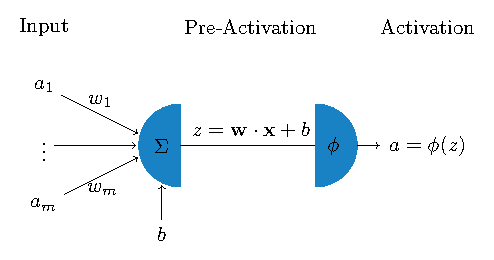
\includegraphics[width=0.5\textwidth]{single_neuron}
    \caption{A single node of a neural network. To get the activation $a$ of the node, the pre-activation $z$ is calculated from the inputs $a_i$ and the bias $b$ and is passed through an activation function $\phi$.}
    \label{fig:single-neuron}
\end{figure}
Before we can build a neural network out of nodes, we have to define how a single node works.
Each node receives the activations $a_i$ from the nodes of the previous layer as inputs.
Each connection is assigned a weight $w_i$, stored in the node's weight vector $\bm{w}$.
\\
Additionally, each node has a so-called \textit{bias} $b$.
The bias shifts the net input of the node by a constant value.
It is needed to model certain problems where part of the prediction is independent of the input \cite[6]{aggarwal_neural_2018}.
Examples include all problems where the output should not be zero even if all inputs are zero.


The net input, called \textit{pre-activation value} $z$ of a node, is the weighted sum of all inputs plus the bias:
\begin{equation}
    z = \sum_{i=1}^{m} w_i a_i + b = \bm{w} \cdot \bm{a} + b \text{.}
    \label{eq:pre-activation}
\end{equation}
The pre-activation value is then passed through an \textit{activation function} $\phi$ to get the activation $a$ of the node, which is then passed on to the next layer, where the process is repeated:
\begin{equation}
    a = \phi(z) \text{.}
    \label{eq:activation}
\end{equation}
The whole process is illustrated in figure \ref{fig:single-neuron}.

\subsection{Activation Functions}
\label{subsec:activation-functions}
The activation function $\phi$ is used to introduce non-linearity into the network and thus increase its modeling power \cite[section 1.2.1.3]{aggarwal_neural_2018}.
Some activation functions are also referred to as \textit{squashing function}~\cite[10]{haykin_neural_1998}, as they map the unbounded pre-activation value $z$ to a bounded activation value $a$.
The choice of activation function has a large impact on the performance of the network in terms of both accuracy and speed \cite{dubey_activation_2022}.
The type of function heavily influences the way that information is processed by the network and the complexity of the function naturally has a large impact on the computational cost of the network.
The best choice therefore depends on the problem that is being solved and the architecture of the network.
Typically, the same activation function is used for all nodes in a layer and is applied to the pre-activation value of each node individually, but different layers can use different activation functions depending on their purpose \cite[174]{goodfellow_deep_2016}.
For a long time, the most popular activation functions were \cite[chapter 6.3]{goodfellow_deep_2016}\cite[section 1.2.1.3]{aggarwal_neural_2018} the sigmoid function:
\begin{equation}
    \phi(z) = \sigma(z) = \frac{1}{1+e^{-z}}
    \label{eq:sigmoid}
\end{equation}
and the hyperbolic tangent function:
\begin{equation}
    \phi(z) = \tanh(z) = \frac{e^z - e^{-z}}{e^z + e^{-z}} = 2\sigma(2z) - 1
    \label{eq:tanh}
\end{equation}
as well as the sign function:
\begin{equation}
    \phi(z) = \text{sign}(z) = \begin{cases}
        1 & \text{if } z > 0 \\
        0 & \text{if } z = 0 \\
        -1 & \text{if } z < 0 \text{.}
    \end{cases}
    \label{eq:sign}
\end{equation}
The sign function can map neural network output to a binary classification, but it is not suitable for backpropagation (see section \ref{subsec:backprop}) due to its derivative being zero almost everywhere.
The sigmoid function and the hyperbolic tangent function are both differentiable and limit the output to the range $(-1, 1)$ and $(0, 1)$ respectively.
They are however more computationally expensive than other activation functions and suffer from the \textit{vanishing gradient problem}.
The vanishing gradient problem describes the fact that the derivative of the sigmoid function approaches zero for large absolute values of $z$.
This leads to the weights of the nodes in the first layers of the network being updated very slowly, as the gradient of the loss function with respect to the weights of these nodes is very small (see section \ref{subsec:backprop})\cite[section 1.4.2]{aggarwal_neural_2018}\cite{dubey_activation_2022}.
The sigmoid function and the hyperbolic tangent function can be seen in figure \ref{fig:sigmoid} and \ref{fig:tanh}.
\begin{figure}
    \centering
    \begin{subfigure}[b]{0.45\textwidth}
        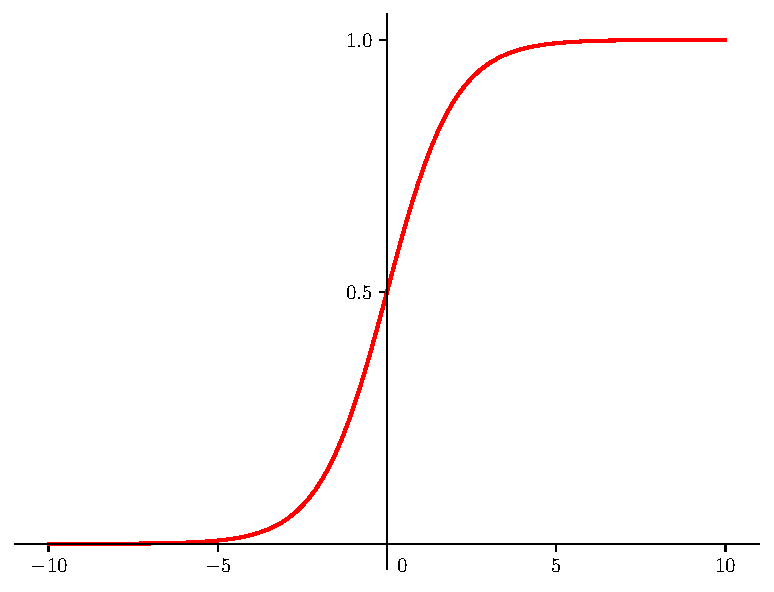
\includegraphics[width=\textwidth]{sigmoid}
        \caption{The sigmoid activation function.}
        \label{fig:sigmoid}
    \end{subfigure}
    \hfill
    \begin{subfigure}[b]{0.45\textwidth}
        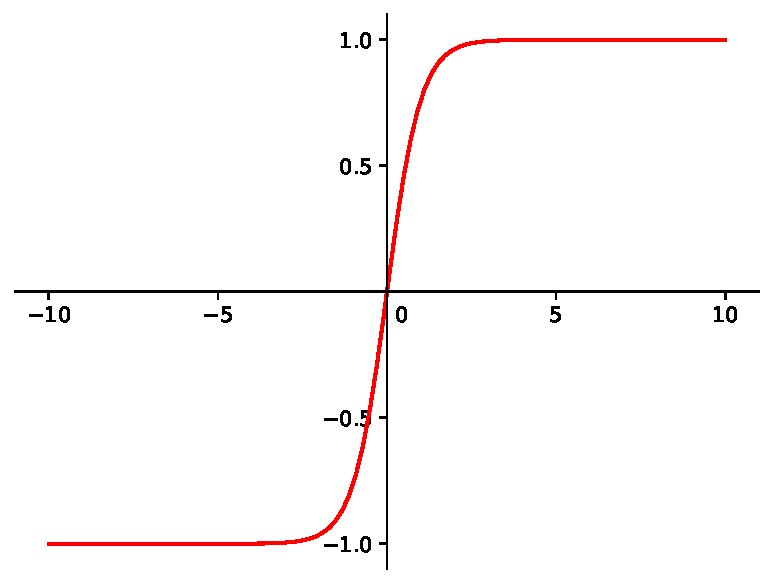
\includegraphics[width=\textwidth]{tanh}
        \caption{The hyperbolic tangent activation function.}
        \label{fig:tanh}
    \end{subfigure}
    \caption{The most popular activation functions before the rise of ReLU.}
    \label{fig:tanhsigmoid}
\end{figure}


In recent years, the \textit{rectified linear unit} (ReLU) and similar stepwise linear functions have become the go-to activation functions for deep neural networks~\cite[chapter 6.3.2]{goodfellow_deep_2016}\cite{dubey_activation_2022}.
ReLU is defined as:
\begin{equation}
    \phi(z) = \max(0, z) = \begin{cases}
        0 & \text{if } z \leq 0 \\
        z & \text{if } z > 0 \text{.}
    \end{cases}
    \label{eq:relu}
\end{equation}
Its main advantage is its very low computational cost, as it consists of only a single comparison.
Although it is not as prone to the vanishing gradient problem as the sigmoid and the hyperbolic tangent, the problem still exists for negative values of $z$.
This has been addressed by variations like \textit{Leaky ReLU}, introducing a small but non-zero slope for negative values~\cite{dubey_activation_2022}:
\begin{equation}
    \phi(z) = \max(0.01 z, z) = \begin{cases}
        0.01 z & \text{if } z \leq 0 \\
        z & \text{if } z > 0 \text{.}
    \end{cases}
    \label{eq:leaky-relu}
\end{equation}
The ReLU function and its leaky version can be seen in figures \ref{fig:relu} and \ref{fig:leaky-relu}.
\begin{figure}
    \centering
    \begin{subfigure}[b]{0.45\textwidth}
        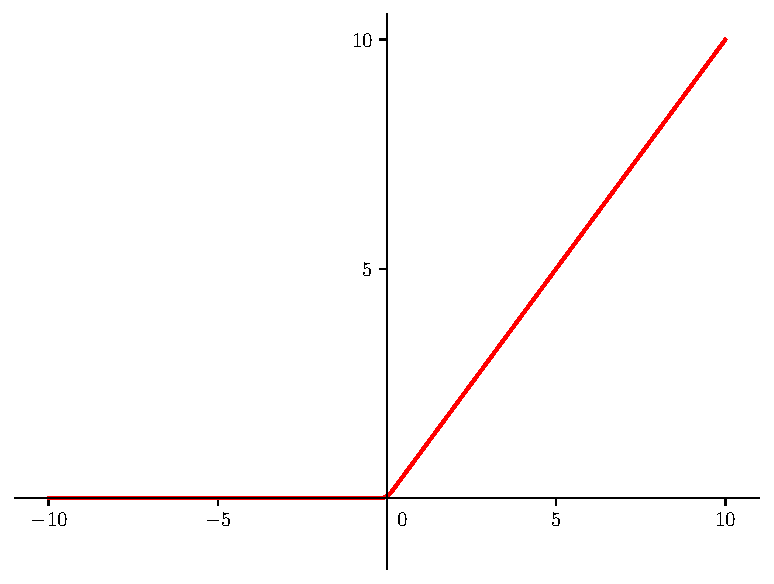
\includegraphics[width=\textwidth]{relu.pdf}
        \caption{The rectified linear unit (ReLU) activation function.}
        \label{fig:relu}
    \end{subfigure}
    \hfill
    \begin{subfigure}[b]{0.45\textwidth}
        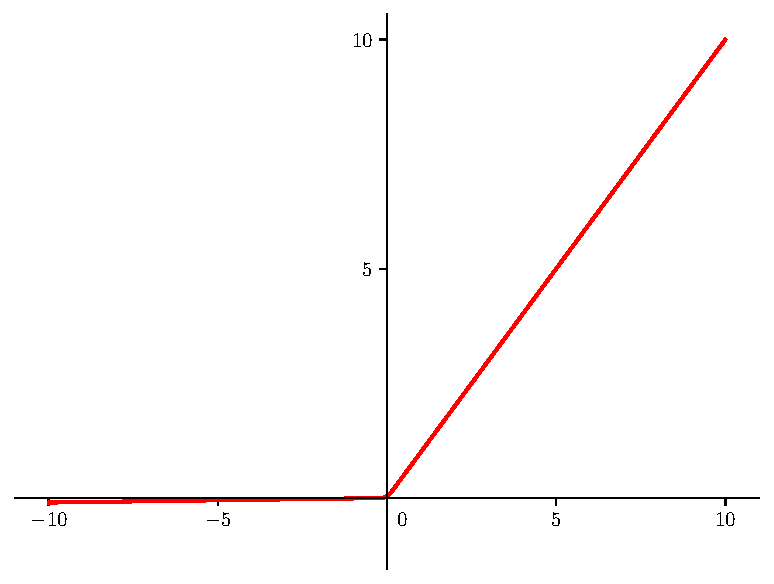
\includegraphics[width=\textwidth]{leaky_relu.pdf}
        \caption{The leaky rectified linear unit (Leaky ReLU) activation function.}
        \label{fig:leaky-relu}
    \end{subfigure}
    
    \caption{Modern, stepwise linear activation functions.}
    \label{fig:subfigures}
\end{figure}


\subsection{Forward-Propagation in Feedforward Neural Networks}
\label{subsec:forward-propagation}
\begin{figure}
    \centering
    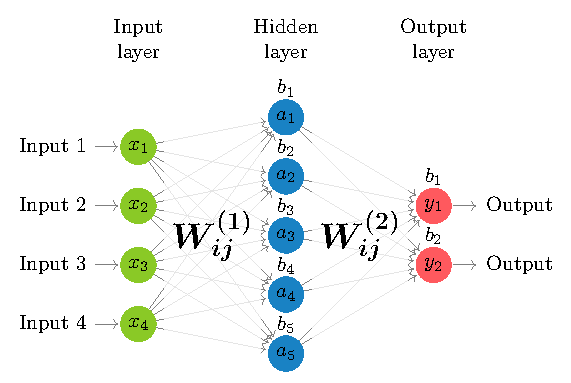
\includegraphics[width=0.9\textwidth]{nn}
    \caption{A feedforward neural network with one hidden layer.}
    \label{fig:nn}
\end{figure}
Now that the workings of the nodes are defined, we can build a fully connected neural network out of these building blocks.
I will illustrate the process using the example of a feedforward neural network as defined in section \ref{sec:overview}.
An example of such a network can be seen in figure \ref{fig:nn}.


The process of feeding an input vector $\bm{x}$ through the network to get the output vector $\bm{y}$ is called \textit{forward-propagation}, as the information propagates through the network's layers.
The activation of any layer $\bm{a}^{[J]}$ can be calculated from the activation of the previous layer $\bm{a}^{[J-1]}$ by generalizing equation \ref{eq:pre-activation} and \ref{eq:activation} to the vector case:
\begin{equation}
    z_k^{[J]} = \sum_{i=1}^{m} w_{ki}^{[J]} a_i^{[J-1]} + b_k^{[J]} \implies \bm{z}^{[J]} = W^{[J]} \bm{a}^{[J-1]} + \bm{b}^{[J]} \text{,}
    \label{eq:pre-activation-vector}
\end{equation}
\begin{equation}
    a_k^{[J]} = \phi(z_k^{[J]}) \implies \bm{a}^{[J]} = \phi(\bm{z}^{[J]}) \text{,}
    \label{eq:activation-vector}
\end{equation}
where the activation function $\phi: \mathbb{R}^m \rightarrow \mathbb{R}^m$ is applied element-wise.
The activation of the input layer $\bm{a}^{[0]}$ is simply the input vector $\bm{x}$ and the activation of the output layer $\bm{a}^{[L]}$ is the output vector $\bm{y}$.


Equations \ref{eq:pre-activation-vector} and \ref{eq:activation-vector} can be applied recursively to calculate the activation of each layer from the input layer to the output layer:
\begin{align}
    \bm{y} = \bm{a}^{[L]} &= \phi(W^{[L]} \bm{a}^{[L-1]} + \bm{b}^{[L]}) \\
    &= \phi(W^{[L]} \phi(W^{[L-1]} \bm{a}^{[L-2]} + \bm{b}^{[L-1]}) + \bm{b}^{[L]}) \\
    &= \phi(W^{[L]} \phi(W^{[L-1]} \phi(\dots \phi(W^{[1]} \bm{x} + \bm{b}^{[1]}) \dots) + \bm{b}^{[L-1]}) + \bm{b}^{[L]}) \text{.}
    \label{eq:forward-propagation}
\end{align}
This equation also shows the significance of the activation function.
Without it, the whole network would be equivalent to a single layer and could be replaced by a single matrix multiplication.
It would therefore only be able to model linear functions.
To show this, let's set $\phi(z)$ to the identity in equation \ref{eq:forward-propagation}.
This yields:
\begin{align}
    \bm{y} &= W^{[L]} W^{[L-1]} \dots W^{[1]} \bm{x} + \bm{b}^{[L]} + W^{[L]} \bm{b}^{[L-1]} + \dots + W^{[L]} W^{[L-1]} \dots W^{[2]} \bm{b}^{[1]} \\
    &= \widetilde{W} \bm{x} + \tilde{\bm{b}} \text{.}
    \label{eq:linear-network}
\end{align}

\subsection{Loss Functions and Gradient Descent}
\label{subsec:loss-functions}
In order to produce meaningful output, the network's weights and biases have to be adjusted to minimize the error of the network's output.
This process is called \textit{training} the network.
The error of the network is measured by a \textit{loss function} $\lambda(\bm{y}, \bm{\hat{y}})$, where $\bm{\hat{y}}$ is some target output vector.
The loss function is a measure of how far the network's output $\bm{y}$ is from the target output $\bm{\hat{y}}$.
As we want to minimize the network's error, the training process is essentially an optimization problem \cite[chapter 4.3]{goodfellow_deep_2016}.
Let's step back from neural networks for a moment and look at a method to minimize a function $f(\bm{x})$ with respect to its parameters $\bm{x}$.
The most common method to do this in machine learning is \textit{gradient descent} \cite[chapter 4.3]{goodfellow_deep_2016}.


\begin{figure}
    \centering
    \begin{subfigure}[b]{0.45\textwidth}
        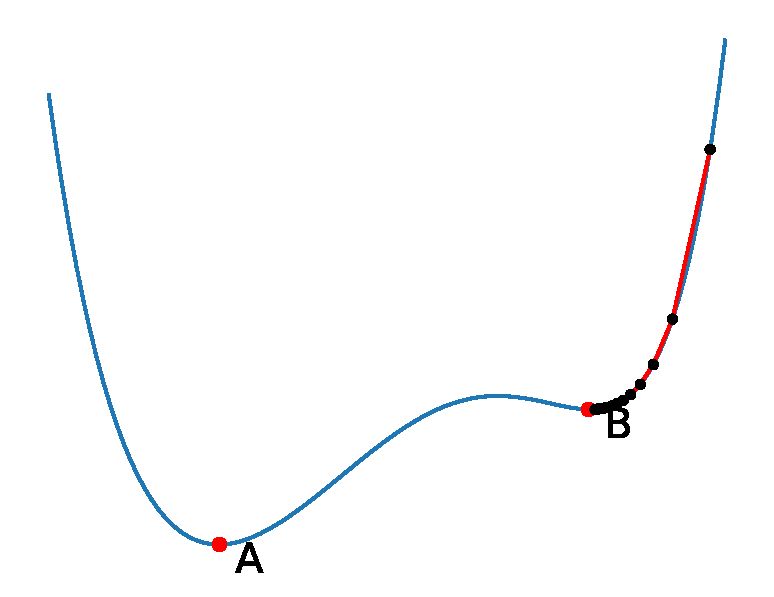
\includegraphics[width=\textwidth]{gradient_descent_small_lr}
        \caption{Gradient descent with a small learning rate.}
        \label{fig:gradient-descent-small}
    \end{subfigure}
    \hfill
    \begin{subfigure}[b]{0.45\textwidth}
        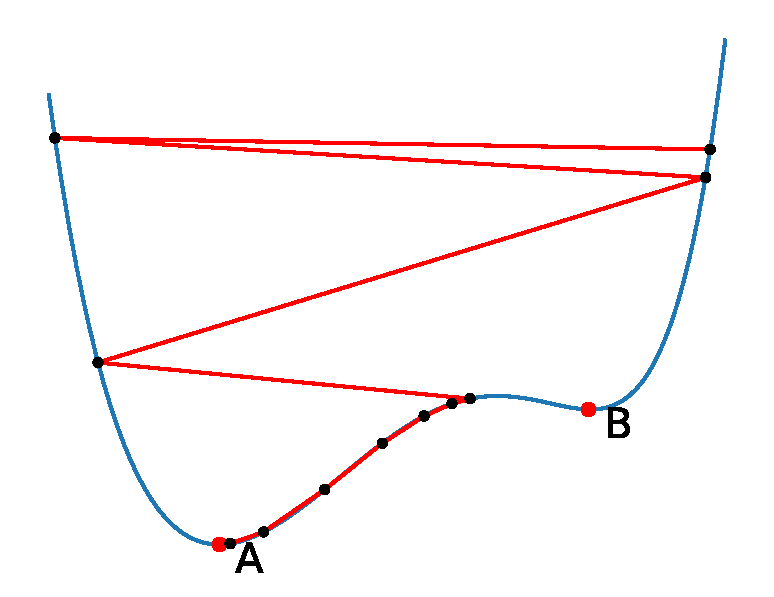
\includegraphics[width=\textwidth]{gradient_descent_large_lr}
        \caption{Gradient descent with a large learning rate.}
        \label{fig:gradient-descent-large}
    \end{subfigure}
    \caption{Gradient descent with different learning rates. Choosing the learning rate too small can lead to slow convergence and to being stuck in local minima. Choosing the learning rate too large can lead to \textit{overshooting} and to the algorithm diverging. Here, the algorithm still converges, but the large oscillations slow down the convergence.}
    \label{fig:gradient-descent}
\end{figure}
If we imagine the function $f(\bm{x})$ as a landscape, the goal of gradient descent is to find the lowest point of the landscape.
To do this, the algorithm starts at some point $\bm{x}_0$ and in each iteration takes a step in the direction of the steepest descent.
The size of the step is determined by the \textit{learning rate} $\eta$.
Choosing an appropriate learning rate is crucial for the algorithm to converge.
Figure \ref{fig:gradient-descent} shows gradient descent with different learning rates and the resulting paths through the landscape.


As is known from multivariable calculus, the direction of the steepest descent of a function $f(\bm{x})$ is given by the negative gradient $\nabla f(\bm{x})$.
We can therefore update the parameters $\bm{x}$ in each iteration by:
\begin{equation}
    \bm{x}_{n+1} = \bm{x}_n - \eta \nabla f(\bm{x}_n) \text{.}
    \label{eq:gradient-descent}
\end{equation}
After a sufficient number of iterations, the algorithm will converge to a local minimum of the function.
In the region around the minimum, the gradient is close to zero and the algorithm will not change the parameters significantly anymore.
We therefore define a threshold $\epsilon$ and stop the algorithm if the norm of the gradient falls below this threshold.
The gradient descent algorithm is summarized in algorithm \ref{alg:gradient-descent}.
\begin{algorithm}
    \caption{Gradient Descent}
    \label{alg:gradient-descent}
    \begin{algorithmic}[1]
        \renewcommand{\algorithmicensure}{\textbf{Output:}}
        \Require
            \Statex $f(\bm{x})$: Function to minimize
            \Statex $\eta$: Learning rate
            \Statex $\epsilon$: Threshold
            \Statex $\bm{x}_0$: Initial parameters
        \Ensure $\bm{x^*}=\arg\min f(\bm{x})$: Parameters that minimize $f(\bm{x})$
        \output{$\bm{x\star}=\arg\min f(\bm{x})$: Parameters that minimize $f(\bm{x})$}
        \Statex
        \State $\bm{x} \gets \bm{x}_0$ \Comment{Initialize parameters}
        \While{$\norm{\nabla f(\bm{x})} > \epsilon$} \Comment{Until convergence}
            \State $\bm{x} \gets \bm{x} - \eta \nabla f(\bm{x})$ \Comment{Update parameters}
        \EndWhile
        \State \Return $\bm{x}$ \Comment{Return parameters}
    \end{algorithmic}
\end{algorithm}

Going back to neural networks, the function that we want to minimize is the loss function $\lambda(\bm{y}, \bm{\hat{y}})$.
As the loss function depends on the network's output $\bm{y}$, which in turn depends on the network's parameters $\bm{w}$ and $\bm{b}$, the loss function is a function of the network's parameters $\lambda(\bm{w}, \bm{b})$.


For single-layer networks, the calculation of the gradients is straightforward.
For multi-layer networks, however, the loss function depends on the parameters of earlier layers in a non-trivial way.
The next section will outline an algorithm that allows the efficient calculation of the gradients of multi-layer networks.

\subsection{The Backpropagation Algorithm}
\label{subsec:backprop}
The calculation of the gradients is the most computationally expensive part of training a neural network.
The invention of the \textit{backpropagation} algorithm by Rumelhart et al. in 1986~\cite{rumelhart_learning_1986} was a major breakthrough in the field of neural networks, as it allowed very efficient gradient calculation and thus enabled the training of large neural networks.
\\
The idea behind backpropagation is to propagate the error back through the network after each forward-propagation step using so-called \textit{local gradients} $\delta$.
During the forward-propagation step, the activations of each layer are stored in memory and later used to calculate the derivatives needed for the backpropagation step.
This is a form of \textit{automatic differentiation}~\cite{adams_backprop_autodiff_nodate,rall_autodiff_1981} and allows the calculation of the gradients with the same time complexity as the forward-propagation step.
This is sometimes called the \textit{cheap gradient principle}~\cite{griewank_derivatives_2008}.
The following mathematical derivation of the backpropagation algorithm is based on~\cite[chapter 4.4]{haykin_neural_1998} as well as~\cite[chapter 6.5]{goodfellow_deep_2016}.


To calculate the update of a weight $w_{ij}^{[K]}$, we have to calculate the derivative of the loss function $\lambda$ with respect to the weight $w_{ij}^{[K]}$:
\begin{equation}
    \Delta w_{ij}^{[K]} = \eta \cdot \frac{\partial \lambda}{\partial w_{ij}^{[K]}} \text{.}
    \label{eq:weight-derivative} 
\end{equation}
This derivative can be evaluated using the chain rule:
\begin{equation}
    \frac{\partial \lambda}{\partial w_{ij}^{[K]}} = \frac{\partial \lambda}{\partial a_i^{[K]}} \frac{\partial a_i^{[K]}}{\partial z_i^{[K]}} \frac{\partial z_i^{[K]}}{\partial w_{ij}^{[K]}} \eqqcolon \delta_i^{[K]} a_j^{[K-1]} 
    \label{eq:chain-rule}
\end{equation}
where we used equation \ref{eq:pre-activation-vector} to simplify the last derivative and defined the local gradient $\delta_j^{[K]}$ as:
\begin{equation}
    \delta_i^{[K]} \coloneqq \frac{\partial \lambda}{\partial a_i^{[K]}} \frac{\partial a_i^{[K]}}{\partial z_i^{[K]}} \text{.}
    \label{eq:local-gradient}
\end{equation}
Let's take a closer look at the local gradient $\delta_i^{[K]}$.
The second factor in equation \ref{eq:local-gradient} is the derivative of the activation function $\phi$ with respect to the pre-activation value $z_i^{[K]}$.
This term is straightforward to calculate.
Remembering that the activation function is applied element-wise, using equation \ref{eq:activation-vector} we get:
\begin{equation}
    \frac{\partial a_i^{[K]}}{\partial z_i^{[K]}} = \frac{\partial \phi(z_i^{[K]})}{\partial z_i^{[K]}} = \phi'(z_i^{[K]}) \text{.}
    \label{eq:activation-derivative}
\end{equation}
The first factor in equation \ref{eq:local-gradient} is the derivative of the loss function $\lambda$ with respect to the activation $a_i^{[K]}$.
If layer $K$ is the output layer, this derivative is simply the derivative of the loss function with respect to the output value $y_i$:
\begin{equation}
    \frac{\partial \lambda}{\partial a_i^{[K]}} = \frac{\partial \lambda}{\partial y_i} \text{.}
    \label{eq:loss-derivative-output}
\end{equation}
If layer $K$ is not the output layer, the derivative is slightly more complicated.
We can use the chain rule trick again, re-introducing the activation values $a_n^{[K+1]}$ of the next layer, which all depend on $a_i^{[K]}$:
\begin{equation}
    \frac{\partial \lambda}{\partial a_i^{[K]}} = \sum_{n=1}^{m_{K+1}} \frac{\partial \lambda}{\partial a_n^{[K+1]}} \frac{\partial a_n^{[K+1]}}{\partial a_i^{[K]}} = \sum_{n=1}^{m_{K+1}} \frac{\partial \lambda}{\partial a_n^{[K+1]}} \frac{\partial a_n^{[K+1]}}{\partial z_n^{[K+1]}} \frac{\partial z_n^{[K+1]}}{\partial a_i^{[K]}} \text{.}
    \label{eq:loss-derivative-hidden}
\end{equation}
Similar to equation \ref{eq:chain-rule}, we can use equation \ref{eq:pre-activation-vector} to simplify the last derivative and identify the local gradients $\delta_n^{[K+1]}$: 
\begin{equation}
    \frac{\partial \lambda}{\partial a_i^{[K]}} = \sum_{n=1}^{m_{K+1}} \delta_n^{[K+1]} w_{ni}^{[K+1]} \text{.}
    \label{eq:loss-derivative-hidden-simplified}
\end{equation}
Plugging equations \ref{eq:activation-derivative} and \ref{eq:loss-derivative-output} or \ref{eq:loss-derivative-hidden-simplified} back into equation \ref{eq:local-gradient} yields the final form of the local gradient:
\begin{equation}
    \delta_i^{[K]} = \phi'(z_i^{[K]}) \cdot \begin{cases}
         \frac{\partial \lambda}{\partial y_i} & \text{if layer } K \text{ is the output layer} \\
         \sum_{n=1}^{m_{K+1}} \delta_n^{[K+1]} w_{ni}^{[K+1]} & \text{otherwise} \text{.}
    \end{cases}
    \label{eq:local-gradient-final}
\end{equation}
This equation can be applied recursively to calculate the local gradients of all layers from the output layer to the input layer.
The weight update $\Delta w_{ij}^{[K]}$ can then be calculated using equation \ref{eq:weight-derivative} and \ref{eq:local-gradient-final}:
\begin{equation}
    \Delta w_{ij}^{[K]} = \eta \cdot \delta_i^{[K]} a_j^{[K-1]} \text{.}
    \label{eq:weight-update}
\end{equation}
When introducing the backpropagation algorithm, I summarized it as a method of \textit{propagating the error back through the network}.
The recursive usage of equation \ref{eq:local-gradient-final} is exactly that: We start at the output layer and calculate the local gradients of all nodes in the output layer using equation \ref{eq:local-gradient-final}.
Then we use these local gradients to calculate the local gradients of the previous layer using equation \ref{eq:local-gradient-final} again and so on until we reach the input layer.
Note that we need to store the activations of each layer in memory during the \textit{forward pass} to calculate the updates during the \textit{backward pass} as mentioned at the beginning of this section.


The derivations for the bias updates are analogous to the weight updates and are therefore omitted here.
The only difference is that the last term in equation \ref{eq:chain-rule} is replaced by $1$ as the bias is not connected to any previous layer.
The algorithm for a whole training step (i.e. one forward pass and one backward pass) is summarized in algorithm \ref{alg:backpropagation}.
\begin{algorithm}
    \caption{One training step of a neural network: Forward- and Backpropagation}
    \label{alg:backpropagation}
    \begin{algorithmic}[1]
        \renewcommand{\algorithmicensure}{\textbf{Output:}}
        \Require
            \Statex $\bm{x}$: Input vector
            \Statex $\bm{\hat{y}}$: Target output vector
            \Statex $\bm{w}$: Weight array containing all weight matrices $\bm{w}^{[K]}$
            \Statex $\bm{b}$: Bias array containing all bias vectors $\bm{b}^{[K]}$
            \Statex $\lambda$: Loss function
            \Statex $\phi$: Activation function
            \Statex $\eta$: Learning rate
        \Ensure Updates the weights $\bm{w}$ and biases $\bm{b}$ of the network in place.
        \Statex
        \State $\bm{a}^{[0]} \gets \bm{x}$ \Comment{Initialize activations}
        \For{$K = 1, \dots, L$} \Comment{Forward-pass}
            \State $\bm{z}^{[K]} \gets \bm{w}^{[K]} \bm{a}^{[K-1]} + \bm{b}^{[K]}$ \Comment{Calculate pre-activations}
            \State $\bm{a}^{[K]} \gets \phi(\bm{z}^{[K]})$ \Comment{Calculate activations}
        \EndFor
        \State $\delta^{[L]} \gets \phi'(\bm{z}^{[L]}) \cdot \frac{\partial \lambda(\bm{a}^{[L]}, \bm{\hat{y}})}{\partial \bm{a}^{[L]}}$ \Comment{Initialize local gradients}
        \For{$K = L, \dots, 1$} \Comment{Backward-pass}
            \State $\Delta \bm{w}^{[K]} \gets \eta \cdot \delta^{[K]} \bm{a}^{[K-1]}$ \Comment{Calculate weight updates}
            \State $\Delta \bm{b}^{[K]} \gets \eta \cdot \delta^{[K]}$ \Comment{Calculate bias updates}
            \State $\delta^{[K-1]} \gets \phi'(\bm{z}^{[K-1]}) \cdot \bm{w}^{[K]T} \delta^{[K]}$ \Comment{Calculate local gradients}
        \EndFor
        \State $\bm{w} \gets \bm{w} - \Delta \bm{w}$ \Comment{Update weights}
        \State $\bm{b} \gets \bm{b} - \Delta \bm{b}$ \Comment{Update biases}
    \end{algorithmic}
\end{algorithm}

\subsection{Gradient Descent Optimization Algorithms}
\label{subsec:sgd}
The gradient descent algorithm outlined in section \ref{subsec:loss-functions} can be implemented in different ways, depending on how the training examples are used. 
\\
\textit{Batch gradient descent} uses the whole training set to calculate the gradient in each iteration \cite{ruder_overview_2017}, making it very accurate, but also computationally expensive. \textit{Stochastic gradient descent} (SGD) on the other hand uses only a single training example to calculate the gradient in each iteration \cite{ruder_overview_2017}. This allows for online learning, where the network is trained efficiently on the fly while it is being used, but it also introduces a lot of noise into the gradient calculation, overshooting the minima. 
\\
\textit{Mini-batch gradient descent} is a compromise between the two, using a small batch of training examples to calculate the gradient in each iteration \cite{ruder_overview_2017}. This combines the efficiency of SGD with the accuracy of batch gradient descent but still has some downsides like getting stuck in saddle points, where the gradient is close to zero, but the function is not at a minimum \cite{ruder_overview_2017}. Furthermore, the learning rate has to be chosen carefully, and the constant learning rate can be problematic for datasets where some features occur more frequently than others \cite{ruder_overview_2017}.


To address these problems, many optimization algorithms have been developed over the years, two of which are important for this thesis:
\\
The \textit{Adam} algorithm \cite{kingma_adam_2017} keeps track of the first and second moments of the gradient (an exponentially decaying average of the past gradients and their squares) and uses them to adapt the learning rate for each parameter individually \cite{kingma_adam_2017,ruder_overview_2017}. This can be seen in analogy to the physical momentum of a ball rolling along the hills and valleys of the loss function landscape. Using momentum dampens the sharp oscillations that can arise when using the pure gradients (\enquote{only the gravitational forces}).
\\
The \textit{AdamW} algorithm \cite{loshchilov_decoupled_2019} is a variation of Adam that introduces slight modifications in order to improve its generalization performance. To prevent overfitting, Adam uses an L2-regularization term that adds a small fraction of the old parameter values to the gradient before updating the parameters. AdamW decouples this weight decay from the gradient calculation and adds it directly to the parameter update, which, according to the authors, improves the generalization performance of the network \cite{loshchilov_decoupled_2019}.


\subsection{Summary}
\label{subsec:nn-summary}
In this chapter, the foundations of neural networks were outlined.
Section~\ref{subsec:single-neuron} started by defining the building blocks of neural networks: The \textit{nodes}.
Section~\ref{subsec:forward-propagation} combined \textit{layers} of these nodes into a \textit{fully connected neural network}.
The specific \textit{architecture} of the network, that is the number of layers, the number of nodes per layer and the \textit{activation functions}, depends on the problem that is being solved.
Later, we will see that in our case of deep Q-learning, the size of the \textit{input vector} is determined by the number of cells that are visible to the agent, and the size of the \textit{output vector} is determined by the number of possible actions that the agent can take.


On this basis, the \textit{forward-propagation} step could be analyzed in detail and the significance of the activation function was explained.
Next, section~\ref{subsec:loss-functions} introduced the \textit{loss function} as a measure of the network's error and the \textit{gradient descent} algorithm was outlined as a method to minimize this error.
Finally, the \textit{backpropagation} algorithm treated in section~\ref{subsec:backprop} provides a way to efficiently compute the gradients needed for gradient descent and enables the \textit{training} of large neural networks.
The whole process of forward-propagation, followed by backpropagation and network parameter updates is summarized in pseudocode in algorithm~\ref{alg:backpropagation}.





\chapter{Deep Q-Learning}
\label{ch:dql}


\section{Reinforcement Learning}
Out of the three main branches of machine learning, \textit{supervised learning}, \textit{unsupervised learning} and \textit{reinforcement learning}, reinforcement learning is the most similar to the way humans learn.
\\
While supervised learning is based on the idea of learning from examples and unsupervised learning is concerned with finding patterns in data \cite{ibm_machine_learning}, reinforcement learning is based on the idea of learning from experience \cite[chapter 1.1]{sutton_reinforcement_nodate}.
In reinforcement learning, the learning agent is not told what action to take but instead has to learn which actions lead to a desired outcome by trial and error.
\\
This framework has led to many successes over the last decades, including computer programs that beat the world's best players in board games like chess, Go, backgammon \cite{silver_mastering_2016,silver_mastering_2017,tesauro_temporal_1995} or even in video games like Atari games \cite{mnih_playing_2013} and Dota 2 \cite{openai_dota_2019}, as well as teaching robots how to walk and handle objects \cite{kober_reinforcement_2013,openai_learning_2019}. In the future, reinforcement learning could be used to teach large language models like the one behind ChatGPT logical reasoning, potentially paving the way for artificial general intelligence, as is the subject of current speculations about OpenAI's $Q^*$ model \cite{mit_unpacking_qstar,mcintosh_google_qstar_2023}.

\subsection{Overview}
In a reinforcement learning scenario, the \textit{agent} observes some information about the \textit{environment}, called the \textit{state} of the environment.
It then uses its \textit{policy} to map the state to an \textit{action} that it takes in the environment.
As a reaction, the environment returns a \textit{reward} to the agent and transitions to a new state \cite{openai_spinning_up_rl_intro}.
\\
During the learning process, the agent tries to find a policy that maximizes the total reward that it receives from the environment.
Depending on the type of problem, the agent can either try to maximize the reward in the short term or in the long term.


The following sections will refine these concepts and introduce the formalism of reinforcement learning.

\subsection{Notation}
\label{subsec:notation}
Before diving into the details of reinforcement learning, I will introduce the notation that will be used throughout the following sections.
It is mostly identical to the notation used in \cite{sutton_reinforcement_nodate}.
Some of these definitions might seem a bit abstract at first, but they will become clearer in the following sections, where they are introduced and explained one by one.

\begin{itemize}
    \item $s_t$: The state of the environment at time step $t$.
    \item $a_t$: The action taken by the agent at time step $t$, based on the state $s_t$.
    \item $r_t$: The reward returned by the environment at time step $t$, based on the state $s_t$, action $a_t$ and the new state $s_{t+1}$.
    \item $\pi$: The policy of the agent, mapping states to actions.
    \item $\pi(a|s)$: The probability of the agent taking action $a$ in state $s$.
    \item $p(s_{t+1} | s_t, a_t)$: The probability of the environment transitioning to state $s_{t+1}$ after the agent takes action $a_t$ in state $s_t$.
    \item $\tau$: A trajectory, i.e. a sequence of states, actions and rewards $(s_0, a_0, r_0, s_1, a_1, r_1, \dots)$.
    \item $G_t$: The return at time step $t$, i.e. the total discounted reward from time step $t$ onwards.
    \item $\gamma$: The discount factor, determining how much future rewards are worth compared to immediate rewards.
    \item $v_\pi(s)$: The value of state $s$ under policy $\pi$, i.e. the expected return when starting in state $s$ and following policy $\pi$.
    \item $q_\pi(s, a)$: The value of taking action $a$ in state $s$ under policy $\pi$, i.e. the expected return when starting in state $s$, taking action $a$ and then following policy $\pi$.
    \item $\pi_*, v_*, q_*$: The optimal policy, value function and action-value function respectively.
\end{itemize}


\subsection{Important Concepts}

\subsubsection{Markov Decision Processes}
\label{subsubsec:mdp}
\begin{figure}[h]
    \centering
    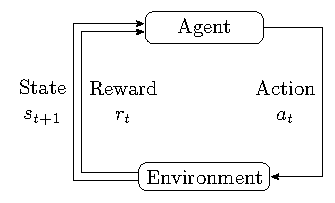
\includegraphics[width=0.5\textwidth]{agent_env_interface.pdf}
    \caption{The agent-environment interface in a Markov decision process as defined in \cite[chapter 3.1]{sutton_reinforcement_nodate}. The agent observes the state $s_t$ of the environment and takes an action $a_t$. The environment transitions to a new state $s_{t+1}$ and returns a reward $r_{t}$ to the agent.}
    \label{fig:agent-env-interface}
\end{figure}
Markov decision processes (MDPs) are a mathematical framework for modeling decision-making in situations where outcomes are partly random and only partly under the control of the agent \cite[chapter 3]{sutton_reinforcement_nodate}.
In an MDP, the agent's actions influence not only the immediate reward but also the next state of the environment and therefore all future rewards.
They are a powerful abstraction that can be used to model a wide range of problems, from simple board games to complex real-world scenarios.
\\
MDPs can be seen as a generalization of discrete-time \textit{Markov chains} (introduced in section \ref{sec:stochastic-processes}), where the next state of the system is determined only by the current state and not by any previous states.
This property is called the \textit{Markov property} and can be expressed in the notation of this chapter as \cite{serfozo_markov_2009}:
\begin{equation}
    p(s_{t+1} | s_1, \dots, s_t) = p(s_{t+1} | s_t) = p_{ss'} \text{.}
    \label{eq:markov-property}
\end{equation}
It is intuitive that the state trajectories in a reinforcement learning scenario should always satisfy this property, as it allows the agent to make decisions based on the current state without having to consider the whole history of states that led to the current state.


MDPs slightly modify the definition of Markov chains by introducing the notion of actions and rewards.
As outlined in the previous section, the agent interacts with the environment by taking actions $a_i$ based on the current state of the environment $s_i$ and receives rewards $r_i$ from the environment in return.
This \textit{agent-environment interface} is illustrated in figure \ref{fig:agent-env-interface}.
A \textit{trajectory} $\tau$ in an MDP is a sequence of states, actions and rewards \cite[48]{sutton_reinforcement_nodate}:
\begin{equation}
    \tau = (s_0, a_0, r_0, s_1, a_1, r_1, s_2, \dots) \text{.}
    \label{eq:trajectory}
\end{equation}
The transition probability now depends on the action $a_t$ that the agent takes in state $s_t$:
\begin{align}
    p: \mathcal{S} \times \mathcal{R} \times \mathcal{S} \times \mathcal{A} &\rightarrow [0, 1] \nonumber \\
    s_{t+1}, r_t, s_t, a_t &\mapsto p(s_{t+1}, r_t | s_t, a_t) \text{,}
    \label{eq:transition-probability}
\end{align}
where $\mathcal{S}$ denotes the set of all possible states and $\mathcal{A}$ denotes the set of all possible actions.\\
This probability function completely determines the dynamics of the reinforcement learning environment.
Environments can be entirely deterministic, entirely stochastic, or anything in between.
The four-argument transition probability, if known, can of course be used to calculate other properties of the environment, such as the three-argument state-transition probability \cite[49]{sutton_reinforcement_nodate}:
\begin{align}
    p: \mathcal{S} \times \mathcal{S} \times \mathcal{A} &\rightarrow [0, 1] \nonumber \\
    s_{t+1}, s_t, a_t &\mapsto p(s_{t+1} | s_t, a_t) = \sum_{r_t \in \mathcal{R}} p(s_{t+1}, r_t | s_t, a_t) \text{.}
    \label{eq:state-transition-probability}
\end{align}
where $\mathcal{R}$ denotes the set of all possible rewards.


Furthermore, knowing the four-argument transition probability of an environment allows us to create a simulation of the environment, which can be used to test reinforcement learning algorithms.
This is a very useful property, as it allows us to test reinforcement learning algorithms in a controlled environment before deploying them in the real world.

\subsubsection{Reward}
After each time step $t$, the agent receives a reward $r_t$ from the environment.
The reward is a scalar value that indicates how good or bad the action $a_t$ that the agent took in state $s_t$ was \cite[53]{sutton_reinforcement_nodate}.
Rewards are the \enquote{trainer's} way of telling the agent what it should achieve.
In order to use the full potential of reinforcement learning, rewards should be chosen carefully.
The reward signal should not tell the agent \textit{how} to achieve the goal, but only \textit{what} the goal is.
The agent should then be able to figure out the best way to achieve the goal by itself \cite[ch. 3.2]{sutton_reinforcement_nodate}.
For example, if the goal is to teach a robot to walk, the agent should receive a reward for moving forward while maintaining a certain balance, but not for moving its legs in a certain way.
\\
In order to be able to learn from these rewards, not just the immediate reward $r_t$ should be taken into account, but also the rewards that the agent will receive in the future.
This is done by introducing the notion of \textit{return}.
The return $G_t$ is a measure of the cumulative reward that the agent will receive from time step $t$ onwards \cite[ch. 3.3]{sutton_reinforcement_nodate}.
The simplest form of return is just the sum of all future rewards:
\begin{equation}
    G_t = r_t + r_{t+1} + r_{t+2} + \dots + r_{T} = \sum_{i=t}^{T} r_{i} \text{,}
    \label{eq:return}
\end{equation}
where $T$ is the final time step in the current \textit{episode}.
Episodic tasks are tasks where a \textit{terminal state} $s_T$ can be reached, after which the episode ends.
Examples are board games like chess or Go, where the game ends after one player wins.
In contrast, for \textit{continuing tasks}, as is the case for the environment that we will consider in this thesis, there is no terminal state and $T=\infty$.
In this case, it's useful to introduce a \textit{discounted} return \cite[ch. 3.3]{sutton_reinforcement_nodate}:
\begin{equation}
    G_t = r_t + \gamma r_{t+1} + \gamma^2 r_{t+2} + \dots = \sum_{i=t}^{\infty} \gamma^{i-t} r_{i} \text{.}
    \label{eq:discounted-return}
\end{equation}
The \textit{discount factor} $\gamma$ determines how much immediate rewards should be valued compared to future rewards.
A discount factor of $\gamma=0$ means that only the immediate reward is taken into account, while a discount factor of $\gamma=1$ would value all future rewards equally.
\\
The discounted reward formula can be rewritten recursively as \cite[55]{sutton_reinforcement_nodate}:
\begin{align}
    G_t &= r_t + \gamma r_{t+1} + \gamma^2 r_{t+2} + \dots \nonumber \\
    &= r_t + \gamma (r_{t+1} + \gamma r_{t+2} + \dots) \nonumber \\
    &= r_t + \gamma G_{t+1} \text{.}
    \label{eq:discounted-return-recursive}
\end{align}
This recursive formulation is very important, as it allows us to express the return in terms of the return at the next time step.
This will be useful in the next sections, where we want to calculate the expected return of a state-action pair.

\subsubsection{Policies}
\label{subsubsec:policies}
Reinforcement learning agents are characterized by their \textit{policy} $\pi$.
The policy maps states $s$ to actions $a=\pi(s)$ and therefore determines the behavior of the agent \cite[ch. 3.5]{sutton_reinforcement_nodate}.
The policy can be either \textit{deterministic} or \textit{stochastic}.
A deterministic policy maps each state to exactly one action, while a stochastic policy maps each state to a probability distribution over actions.
If a policy deterministically maps states to what it believes to be the best action, it is called a \textit{greedy} policy \cite[64]{sutton_reinforcement_nodate}.
If an optimal policy has been found, it can be greedy, as it will always choose the best action.
However, during the learning process, stochastic policies should be preferred, as they allow the agent to explore the environment and find better policies.
In order to learn, an \enquote{inexperienced} agent needs to try actions that it assumes to be suboptimal to find out whether they are really suboptimal.
This is called the \textit{exploration-exploitation dilemma} \cite[3]{sutton_reinforcement_nodate}.\\
A popular solution which will also be used in this thesis is the \textit{$\epsilon$-greedy} policy \cite[100]{sutton_reinforcement_nodate}.
$\epsilon$-greedy policies are greedy with probability $1-\epsilon$ and choose a random action with probability $\epsilon$.
During training, $\epsilon$ is slowly decreased over time, so that the agent will explore the environment more at the beginning and exploit its knowledge later on.
During evaluation, $\epsilon$ is set to zero, so that the agent will always choose the best action.

\subsubsection{Value Functions}
To actually build a policy that maximizes the expected return, the agent needs to know how good each state or state-action pair is. In order to do this, most reinforcement learning algorithms use \textit{(state) value functions} \cite[ch. 3.5]{sutton_reinforcement_nodate}. Value functions estimate the expected return of a state $s$ when following policy $\pi$ \cite[58]{sutton_reinforcement_nodate}:
\begin{equation}
    v_\pi(s) = \mathbb{E}_\pi[G_t | s_t = s] = \mathbb{E}_\pi \left[ \sum_{i=t}^{\infty} \gamma^{i-t} r_{i} \middle| s_t = s \right] \text{.}
    \label{eq:value-function}
\end{equation}
In the same manner, we can define the \textit{action-value function} \cite[58]{sutton_reinforcement_nodate}:
\begin{equation}
    q_\pi(s, a) = \mathbb{E}_\pi[G_t | s_t = s, a_t = a] = \mathbb{E}_\pi \left[ \sum_{i=t}^{\infty} \gamma^{i-t} r_{i} \middle| s_t = s, a_t = a \right] \text{.}
    \label{eq:action-value-function}
\end{equation}


\subsubsection{Optimality and Bellman Equations}
Now the recursion formula from equation \ref{eq:discounted-return-recursive} comes in handy to express the value functions in terms of the value functions of the next state:
\begin{align}
    v_\pi(s) &= \mathbb{E}_\pi[G_t | s_t = s] \nonumber \\
    &= \mathbb{E}_\pi[r_t + \gamma G_{t+1} | s_t = s] \nonumber \\
    &= \sum_a \pi(a|s) \sum_{s'} \sum_{r_t} p(s', r_t | s, a) \left[ r_t + \gamma \mathbb{E}_\pi[G_{t+1} | s_{t+1} = s'] \right] \nonumber \\
    &= \sum_a \pi(a|s) \sum_{s'} \sum_{r_t} p(s', r_t | s, a) \left[ r_t + \gamma v_\pi(s') \right] \text{,}
    \label{eq:bellman-expectation}
\end{align}
where we reintroduced the four-argument transition probability. The summations are over all possible actions $a$ and all possible next states $s'$ and rewards $r_t$. Equation \ref{eq:bellman-expectation} is called the \textit{Bellman equation} for $v_\pi$ \cite[59]{sutton_reinforcement_nodate}.\\
The Bellman equation for $q_\pi$ is analogous \cite{openai_spinning_up_rl_intro}:
\begin{equation}
    q_\pi(s, a) = \sum_{s'} \sum_{r_t} p(s', r_t | s_t, a_t) \left[ r_t + \gamma \sum_{a_{t+1}} \pi(a_{t+1}|s_{t+1}=s') q_\pi(s', a_{t+1}) \right] \text{.}
    \label{eq:bellman-expectation-action-value}
\end{equation}
The Bellman equations heavily simplify the calculation of the value functions, as they allow us to express the value of a state or state-action pair in terms of the values of the next state or state-action pairs.
Imagine a game of chess: Even for very fast computers, evaluating every possible trajectory of moves until one player wins is not feasible.
However, the Bellman equations allow us to calculate the value of a state or state-action pair without having to consider all possible trajectories.
We just have to keep track of the values of individual states or state-action pairs and update them according to the Bellman equations.


We can now use these concepts to define \textit{optimal} policies $\pi_*$. A policy is considered \enquote{better} than another policy if it achieves a higher expected return in every state \cite[62]{sutton_reinforcement_nodate}:
\begin{equation}
    \pi \geq \pi' \Leftrightarrow v_\pi(s) \geq v_{\pi'}(s) \quad \forall s \in \mathcal{S} \text{.}
    \label{eq:policy-ordering}
\end{equation} 
An optimal policy $\pi_*$ is a policy that is better than or equal to all other policies \cite[62]{sutton_reinforcement_nodate}. Associating the value functions $v_*$ and $q_*$ with the optimal policy $\pi_*$, we can define the optimal (action-)value functions as \cite[ch. 3.6]{sutton_reinforcement_nodate}:
\begin{equation}
    v_*(s) = \max_\pi v_\pi(s) \quad \forall s \in \mathcal{S} \text{.}
    \label{eq:optimal-value-function}
\end{equation}
\begin{equation}
    q_*(s, a) = \max_\pi q_\pi(s, a) \quad \forall s \in \mathcal{S}, a \in \mathcal{A} \text{.}
    \label{eq:optimal-action-value-function}
\end{equation}
The optimal value functions satisfy the \textit{Bellman optimality equations} \cite[ch. 3.6]{sutton_reinforcement_nodate}. When an agent follows an optimal policy, the sum over all possible actions can be replaced by using the action that maximizes the expected return:
\begin{align}
    q_*(s, a) &= \mathbb{E}_\pi \left[ r_t + \gamma \max_{a'} q_*(s_{t+1}, a') \middle| s_t = s, a_t = a \right] \nonumber \\
    &= \sum_{s'} \sum_{r_t} p(s', r_t | s, a) \left[ r_t + \gamma \max_{a'} q_*(s', a') \right] \text{.}
    \label{eq:bellman-optimality-action-value}
\end{align}
Solving equation \ref{eq:bellman-optimality-action-value} yields the optimal action-value function $q_*$, which can then be used to derive the optimal policy $\pi_*$. For most reinforcement learning problems, however, it is not feasible to solve the Bellman optimality equations analytically, even if the transition probabilities are known. Therefore, most reinforcement learning algorithms use iterative methods to approximate the optimal value functions \cite[ch. 4]{sutton_reinforcement_nodate}.


\subsection{Summary}
Before we dive into the details of the deep Q-learning algorithm, let's summarize the most important concepts of reinforcement learning that were introduced in this section.


Reinforcement learning is a framework for \textit{learning from experience}.
An \textit{agent} interacts with an \textit{environment} by taking \textit{actions} based on the current \textit{state} of the environment.
The environment returns a \textit{reward} which the agent uses to keep track of the \textit{return} that it will receive in the future.
This in turn allows the agent to learn a \textit{policy} that maximizes the expected return by learning the \textit{value} of each state or state-action pair.
\textit{Optimal} policies can be found by solving the \textit{Bellman optimality equations}.



\subsection{Algorithms}
\label{subsec:rl-algorithms}
\begin{figure}[h]
    \centering
    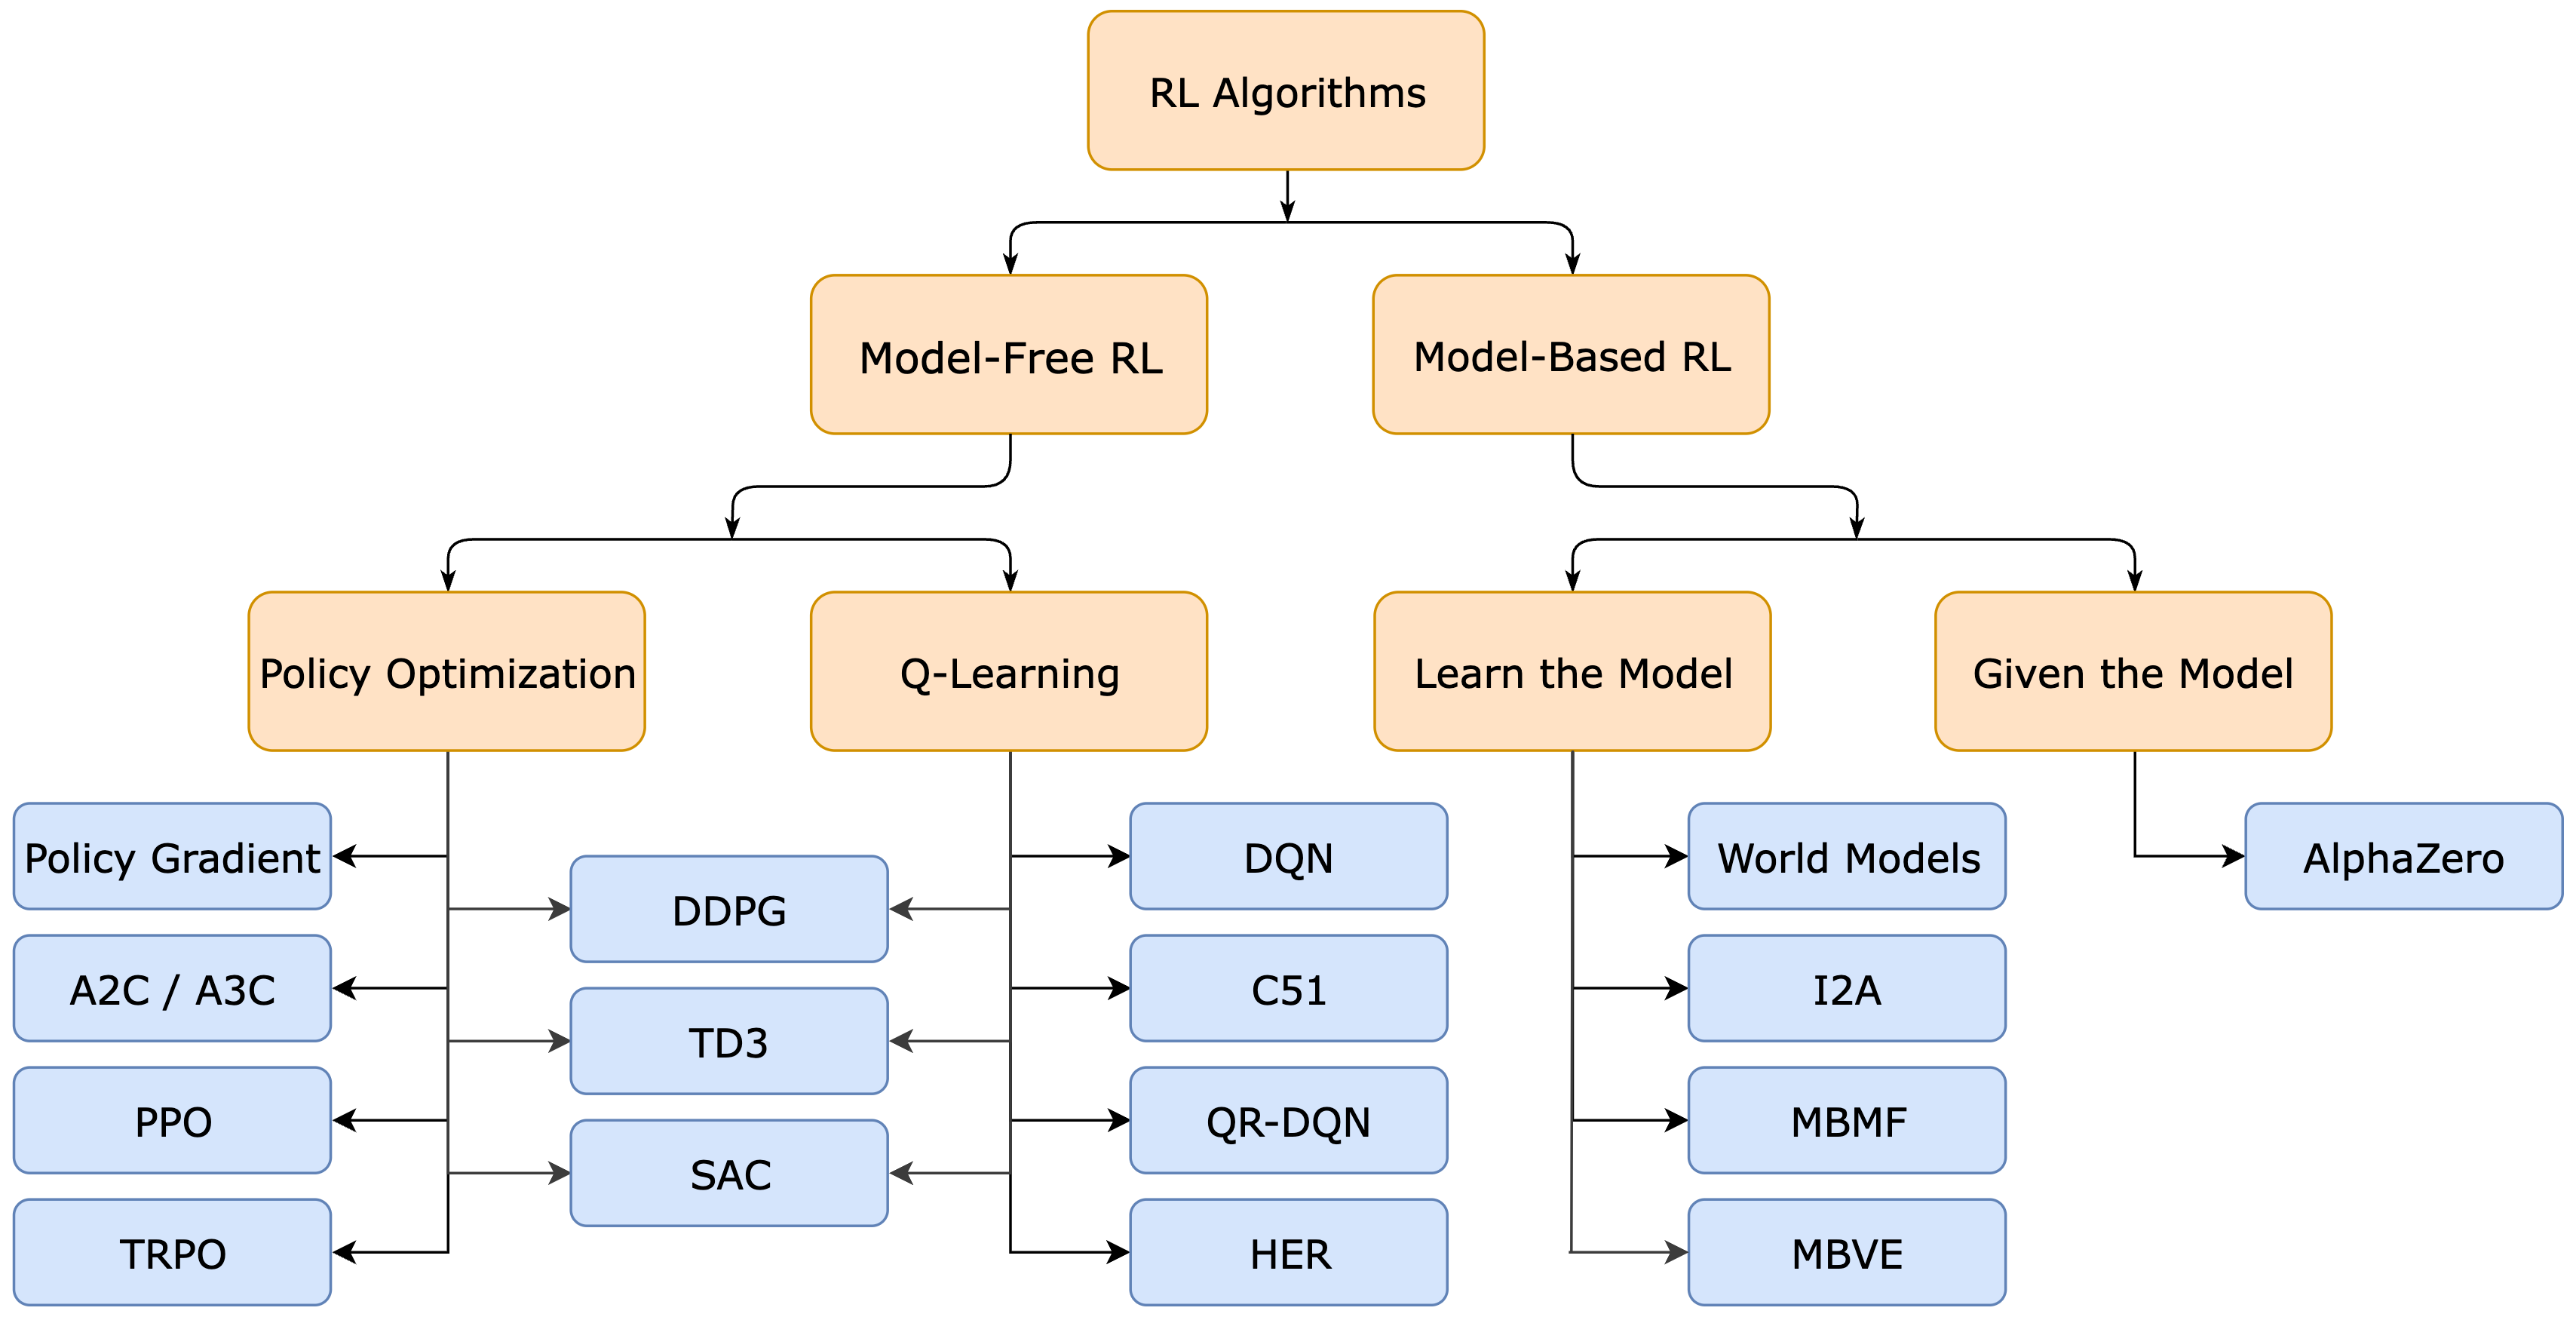
\includegraphics[width=0.8\textwidth]{openai_algorithms}
    \caption{Overview of the different classes of reinforcement learning algorithms \cite{openai_spinning_up_rl_part2}. The papers that introduced the algorithms are also available at \cite{openai_spinning_up_rl_part2}.}
    \label{fig:rl-algorithms}
\end{figure}
Figure \ref{fig:rl-algorithms} provides a basic overview of the different classes of reinforcement learning algorithms. We will not explain the details of each algorithm here but instead focus on the general distinctions between the different classes of algorithms.


The first distinction is between \textit{model-based} and \textit{model-free} algorithms. Model-based algorithms have an internal model of the environment, which is either learned or provided by the user \cite{openai_spinning_up_rl_part2}. This allows them to plan ahead and simulate the environment's dynamics to find the best action to take. Model-free algorithms on the other hand only implicitly learn the dynamics of the environment by interacting with it and learning value functions, as explained in the previous sections. Model-free algorithms are more flexible, as they can be applied to any environment, but they are also less sample-efficient, as they have to learn the dynamics of the environment by trial and error. Model-based algorithms on the other hand can be more sample-efficient, but they are harder to implement and fine-tune to specific problems \cite{openai_spinning_up_rl_part2}. Probably the most famous model-based reinforcement learning algorithm is AlphaZero \cite{silver_mastering_2017}, a program that taught itself to play chess, Go and Shogi at superhuman levels.


Model-free algorithms can be distinguished further by \textit{what} is learned. In the last section, we introduced the concept of value functions. Algorithms that learn value functions are called \textit{value-based} algorithms. If they learn the action-value function $q_\pi$, they are called \textit{Q-learning} algorithms. Most of these algorithms use \textit{off-policy} learning, which means that they learn the value of the optimal policy $\pi_*$ while following a different policy $\pi$ \cite{openai_spinning_up_rl_part2}. This allows them to learn from data that was collected at a previous stage of the training process, making them very sample-efficient. Probably the most famous Q-learning algorithm is deep Q-learning, which we will discuss in detail in the next section.
\\
The other class of model-free algorithms is \textit{policy-based} algorithms. These algorithms directly learn the optimal policy $\pi_*$, instead of learning value functions. Most of these algorithms use \textit{on-policy} learning, restricting them to only learn from data that was collected while following the current policy $\pi$ \cite{openai_spinning_up_rl_part2}. Because of that, they are less sample-efficient than Q-learning algorithms, but they also tend to be more stable, as they directly learn the policy, instead of indirectly learning the policy by learning value functions \cite{openai_spinning_up_rl_part2}. 


As we can see in figure \ref{fig:rl-algorithms}, there are also algorithms that use ideas from different classes of algorithms. In general, it is hard to draw clear distinctions between the different classes of algorithms, as their modular nature allows them to be combined in many ways \cite{openai_spinning_up_rl_part2}.


Choosing the best algorithm for a specific problem is one of the most important steps in applying reinforcement learning to a real-world problem. In this thesis, we will use deep Q-learning, as its use of deep neural networks allows it to scale and generalize well. It is also a model-free, off-policy algorithm, which makes it relatively easy to implement and modify. The sampling efficiency of off-policy learning is also a big advantage, as it allows training the network quickly on normal hardware. 



\section{Q-Learning}
\label{sec:q-learning}
Before diving into the details of the deep Q-learning algorithm, we will introduce the general concepts of Q-learning, building on the concepts of reinforcement learning that were introduced in the previous section.


Q-Learning was introduced by Watkins in 1989 \cite{watkins_learning_1989}. It is a model-free, off-policy algorithm that learns an action-value function $Q(s,a)$ which is guaranteed to converge to the optimal action-value function $q_*$ \cite{watkins_q-learning_1992} \cite[ch. 6.5]{sutton_reinforcement_nodate}
\\
The algorithm works by storing a table of action-values $Q(s,a)$ for each state-action pair $(s,a)$ that the agent has encountered. Such a \textit{Q-table} can be seen in figure \ref{fig:q-table}. In the beginning, the Q-table is initialized randomly. Then, the agent interacts with the environment by taking actions and receiving rewards. The policy used for this interaction is derived from the Q-table for example by choosing the action with the highest action-value in an $\epsilon$-greedy manner. For each sample (state $s$, action $a$, reward $r$, next state $s'$) that the agent encounters, the Q-table is updated according to the following formula \cite[ch. 6.5]{sutton_reinforcement_nodate}:
\begin{equation}
    Q(s, a) \gets Q(s, a) + \eta \left[ r + \gamma \max_{a'} Q(s', a') - Q(s, a) \right] \text{,}
    \label{eq:q-learning-update}
\end{equation}
where $\eta$ is the learning rate and $\gamma$ is the discount factor. Comparing with equation \ref{eq:bellman-optimality-action-value}, we can see that this update rule is an iterative approximation of the Bellman optimality equation for $q_*$. The new approximation of the optimal action-value is a weighted sum of the old approximation and the new information that was gained from the sample, i.e. the immediate reward $r$ and the discounted value of the next action. The learning rate $\eta$ determines how much the new information is weighted compared to the old approximation. The discount factor again $\gamma$ determines how much future rewards are valued compared to immediate rewards.


\begin{figure}[h]
    \centering
    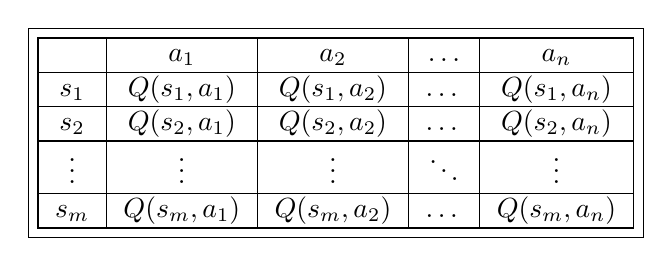
\begin{tikzpicture}
        \node
            (q-table-before)
            [draw]
            {
                \begin{tabular}{|c|c|c|c|c|}
                    \hline
                     & $a_1$ & $a_2$ & $\dots$ & $a_n$ \\
                    \hline
                    $s_1$ & $Q(s_1, a_1)$ & $Q(s_1, a_2)$ & \dots & $Q(s_1, a_n)$ \\
                    \hline
                    $s_2$ & $Q(s_2, a_1)$ & $Q(s_2, a_2)$ & \dots & $Q(s_2, a_n)$ \\
                    \hline
                    $\vdots$ & $\vdots$ & $\vdots$ & $\ddots$ & $\vdots$ \\
                    \hline
                    $s_m$ & $Q(s_m, a_1)$ & $Q(s_m, a_2)$ & \dots & $Q(s_m, a_n)$ \\
                    \hline
                \end{tabular}
            };
    \end{tikzpicture}
    \caption{A Q-table for an environment with $m$ states and $n$ actions.}
    \label{fig:q-table}
\end{figure}
We see that while time complexity stays constant when using lookup tables, the space complexity grows linearly with the number of states and actions. This makes Q-learning impractical for environments with large state spaces. Also, environments that have continuous state or action spaces have to be discretized, which can lead to a loss of information and therefore suboptimal policies. Even for seemingly simple environments such as a grid, where each grid cell can either be occupied or unoccupied, the number of possible states grows exponentially with the size of the grid. Therefore, we need a more efficient way to represent the action-values. This is where deep Q-learning comes in.

\section{Deep Q-Learning}
\label{subsec:deep-q-learning}
To solve the problem of large state spaces, we look back at chapter \ref{ch:neural-networks}, where we learned, that deep neural networks are universal function approximators. This makes them a good candidate for approximating the action-values $Q(s,a)$. When we replace the Q-table with a neural network, we supply the current state $s$ as input and get the action-values $Q(s,a)$ as output. For our grid environment example from the last section, this would mean that we supply the current grid as input. This eliminates the exponential space complexity of the Q-table, as the input vector of the network now grows linearly with the number of cells. Furthermore, the discretization problem is also solved, as the network can now take continuous inputs. Ideally, the network would store the same information as the table, but in a more compact way by learning the patterns in the data.  


This approach is called \textit{deep Q-learning} (DQN) and was introduced by Mnih et al. in 2013 \cite{mnih_playing_2013}. DQN also introduces a few other concepts apart from the Q-network, which we will discuss in the following sections.

\subsection{Q-Network}
\label{subsec:q-network}
The Q-network, sometimes also called \textit{policy network}, was already discussed in the previous section. It is a neural network that replaces the Q-table and approximates the action-values $Q(s,a)$. During evaluation, the environment's state is supplied as input to the network. After a forward pass through the network, as explained in section \ref{subsec:forward-propagation}, the output vector of the network corresponds to the approximate action-values $Q(s,a)$ for each action $a$. When the network has converged to a good approximation of the optimal action-values $q_*$, the action with the highest action-value can be chosen as the action that the agent takes in the current state. During training, this action is chosen in an $\epsilon$-greedy manner, as explained in section \ref{subsubsec:policies} to maintain exploration \cite{mnih_human-level_2015}. 

\subsection{Target Network}
\label{subsec:target-network}
The Q-network also changes the way that the parameters are updated.
We can no longer update individual Q-values, as this information is now encoded in the weights and biases of the network.
Instead, we have to update the parameters of the network.
This is done by using  \textit{gradient descent} and the \textit{backpropagation} algorithm, as explained in sections \ref{subsec:loss-functions} and \ref{subsec:backprop}.


The loss function that is used for the gradient descent requires a target output vector $\hat{y}$ for each sample. In the case of Q-learning, this would be the optimal action-values $q_*(a)$. As this is what we're optimizing for, we can't use it as the target output vector. Instead, we could use an earlier approximation of the action-values $Q(s,a)$. However, this can lead to oscillations or divergence of the network parameters, as the target network would use the same parameters as the Q-network \cite{mnih_human-level_2015}. To solve this problem, DQN introduces a second network, called the \textit{target network}. The target network is a clone of the Q-network with frozen parameters. Using this separate network to calculate the action-value targets makes the learning process more stable \cite{mnih_human-level_2015}.
\\
In the original algorithm, the target network parameters are updated periodically by copying the parameters from the Q-network. This is called \textit{hard target network update} \cite{mnih_human-level_2015}. In 2016, Lillicrap et al. \cite{lillicrap_continuous_2015} introduced \textit{soft target network updates}, where the target network parameters are updated by slowly blending the parameters of the Q-network into the target network parameters:
\begin{equation}
    \theta_{\text{target}} \gets \tau \theta_{\text{Q}} + (1 - \tau) \theta_{\text{target}} \text{,}
    \label{eq:soft-target-update}
\end{equation}
where $\tau\ll1$ is a small number between 0 and 1, $\theta_{\text{target}}$ are the target network parameters and $\theta_{\text{Q}}$ are the Q-network parameters.
\\
This makes the learning process even more stable, as the target network parameters are constrained to slow updates \cite{lillicrap_continuous_2015}. In this thesis, we will also use soft target network updates.

\subsection{Experience Replay}
\label{subsec:experience-replay}
At the beginning of this section, DQN was introduced as an off-policy algorithm. Mnih et al. introduced a technique called \textit{experience replay} \cite{mnih_human-level_2015}, which massively improves the algorithm's quality. The technique is inspired by the way that humans learn \cite{mnih_human-level_2015} and works by storing tuples of states, actions, rewards and next states $(s_t, a_t, r_t, s_{t+1})$, called \textit{transitions} in a \textit{replay buffer}. During training, the network is updated by sampling a batch of transitions from the replay buffer and performing a gradient descent step on the loss function. This not only allows the network to learn from the same experience multiple times, increasing sample efficiency but also breaks up the correlation between consecutive samples, which would otherwise decrease learning efficiency and stability \cite{mnih_human-level_2015}. In order to prevent the replay buffer from growing infinitely, the oldest samples are discarded when the buffer is full. This total buffer size and the sampling batch size are hyperparameters that have to be tuned for each problem. 


% problem rare transitions -> prioritized experience replay
One problem that exists in both on-policy learning and off-policy learning with experience replay is that rare transitions are sampled very infrequently, which can slow down learning. To solve this problem, Schaul et al. introduced \textit{prioritized experience replay} in 2015 \cite{schaul_prioritized_2016}. In prioritized experience replay, each transition is assigned a priority based on the magnitude of the loss function \cite{schaul_prioritized_2016}. That way, transitions that are \enquote{surprising} to the agent are sampled more frequently, which speeds up learning \cite{schaul_prioritized_2016}.

\subsection{Summary}
In this section, we learned that deep Q-learning uses a neural network to map states to action-values. This allows it to scale to large and continuous state spaces. Learning is performed \textit{offline}, by saving encountered transitions to a replay buffer and sampling batches of transitions from the buffer to update the network parameters. A separate target network is used to calculate the action-value targets, which makes the learning process more stable. The target network parameters are updated by slowly blending the parameters of the Q-network into the target network parameters. The complete algorithm is shown in algorithm \ref{alg:dqn}.

\begin{algorithm}[h]
    \caption{Deep Q-Learning}
    \label{alg:dqn}
    \begin{algorithmic}
        \State Initialize replay buffer $\mathcal{D}$ to capacity $N$
        \State Initialize Q-network $Q$ with parameters $\theta$
        \State Initialize target network $\hat{Q}$ with parameters $\theta^-=\theta$
        \State Initialize environment to get initial state $s_1$
        \State Initialize $\epsilon$ to $\epsilon_0$
        \For{steps $t=1,\dots,T$}
            \State $\triangleright$ Generate new transition
            \State Perform forward pass through $Q$ to get action-values $Q(s_t, a')$ 
            \State With probability $\epsilon$ select a random action $a_t$, otherwise select $a_t = \arg\!\max_a Q(s_t, a)$
            \State Execute action $a_t$ in environment and observe reward $r_t$ and next state $s_{t+1}$
            \State Store transition $(s_t, a_t, r_t, s_{t+1})$ in $\mathcal{D}$
            \State $\triangleright$ Update Q-network parameters
            \State Sample random mini-batch of transitions $(\bm{s}, \bm{a}, \bm{r}, \bm{s'})$ from $\mathcal{D}$
            \State Set $\bm{y} = \bm{r} + \gamma \max_{a'} \hat{Q}(\bm{s'}, a')$
            \State Calculate mean loss $\mathcal{L} = \text{mean}(\mathcal{L}(\bm{y}, Q(\bm{s}, \bm{a})))$
            \State Perform gradient descent step on $\mathcal{L}$ using backpropagation and update $\theta$
            \State $\triangleright$ Update target network parameters
            \State Update target network parameters $\theta^- \gets \tau \theta + (1 - \tau) \theta^-$
            \State $\triangleright$ Update exploration rate
            \State Decrease $\epsilon$   
        \EndFor
    \end{algorithmic}
\end{algorithm}








